\documentclass[../Main.tex]{subfiles}

\begin{document}
An important class of potentials (including gravity and electrostatics) depend only on the distance to some origin. The force therefore points towards the origin.
\begin{align*}
    \vec{F} &= -\nabla V = -\frac{dV}{dr} \nabla r \\
    &= - \frac{dV}{dr} \uvec{x}
\end{align*}
\section{Conservation of Angular Momentum}
\begin{definition}{Angular momentum}
    The \underline{angular momentum} of an object relative to the centre of rotation is:
    \begin{equation}
        \vec{L} = m \vec{x} \times \dvec{x}
        \label{eqnAngularMomentum}
    \end{equation}
\end{definition}
Angular momentum is orthogonal to both position and velocity.\par
A key fact about central forces is that angular momentum is conserved.\par
Then we consider how angular momentum changes with time:
\begin{align*}
    \frac{d\vec{L}}{dt} &= m \frac{d}{dt}(\vec{x} \times \dvec{x}) \\
    &= m(\dvec{x} \times \dvec{x} + \vec{x} \times \ddvec{x}) \\
    &= \vec{x} \times \vec{F}
\end{align*}
We define this quantity to be the torque, $\vec{G} = \vec{x} \times \vec{F}$.\par
For a central force, $\vec{F}$ is in the direction of $\vec{x}$, so $\frac{d\vec{L}}{dt} = 0$. This therefore shows that the particle must move in the same plane (the plane orthogonal to $\vec{L}$), since $\vec{L}$ is conserved. Therefore, we have reduced a 3-dimensional problem to a 2-dimensional one.
\section{Polar coordinates}
In the plane orthogonal to $\vec{L}$, consider polar coordinates ($x = r \cos{\theta}, y = r\sin{\theta}$).\par
Then let $\uvec{r}$ be the 2-dimensional vector in the direction of $\vec{x}$, and let $\uvec{{\theta}}$ be the vector perpendicular to it in the plane.
\begin{align*}
    \uvec{r} &= \begin{pmatrix}\cos{\theta} \\ \sin{\theta}\end{pmatrix} \\
    \uvec{\theta} &= \begin{pmatrix}-\sin{\theta} \\ \cos{\theta}\end{pmatrix}
\end{align*}
Recall from IA Vector Calculus that these vectors depend on position.\par
Differentiating the position vector:
\begin{align*}
    \vec{x} &= r \uvec{r} \\
    \dvec{x} &= \dot{r}\uvec{r} + r\duvec{r} \\
    &= \dot{r}\uvec{r} + r \frac{d\uvec{r}}{d\theta} \frac{d\theta}{dt} \\
    &= \dot{r}\uvec{r} + r \dot{\theta}\uvec{\theta} \\
    \ddvec{x} &= \ddot{r} \uvec{r} + 2 \dot{r} \dot{\theta} \uvec{\theta} + r \ddot{\theta} \uvec{\theta} + r \dot{\theta} \uvec{\theta} \\
    &= \left(\ddot{r} - r \dot{\theta}^2\right)\uvec{r} + \left(r\ddot{\theta} + 2 \dot{r}\dot{\theta}\right)\uvec{\theta}
\end{align*}
Then Newton's Second Law in polar coordinates is:
\begin{align}
    \uvec{\theta}: &~r\ddot{\theta} + 2\dot{r}\dot{\theta} = 0 \label{eqnNewtonIIPolar} \\
    \uvec{r}: &~m\left(\ddot{r} - r \dot{\theta}^2\right) = -\frac{dV}{dr} \nonumber
\end{align}
We consider the angular momentum again:
\begin{align*}
    \vec{L} &= m\vec{x} \times \dvec{x} \\
    &= m r \uvec{r} \times \left(\dot{r} \uvec{r} + r \dot{\theta} \uvec{\theta}\right) \\
    &= m r^2 \dot{\theta} (\uvec{r} \times \uvec{\theta})
\end{align*}
And so we define $|\vec{L}| = ml = mr^2 \dot{\theta}$. We often refer to $l$ as the angular momentum, where really it is angular momentum per unit mass.\par
Then we can use $l = r^2 \dot{\theta}$ to simplify equation~\ref{eqnNewtonIIPolar}:
\begin{equation}
    m\ddot{r} - \frac{ml^2}{r^3} = -\frac{dV}{dr} = F(r)
    \label{eqnRadialEquation}
\end{equation}
Then equation~\ref{eqnRadialEquation} is only an equation in $r(t)$, so we have reduced the two-dimensional problem to a single dimension.
\section{The Effective Potential}
To simplify this even further, we define the \underline{effective potential}:
\begin{equation*}
    V_{eff}(r) = V(r) + \frac{ml^2}{2r^2}
\end{equation*}
Such that when differentiated, it satisfies:
\begin{equation}
    m\ddot{r} = -\frac{dV_{eff}}{dr}
    \label{eqnSimplifiedPotential}
\end{equation}
Let $V(r)$ be $-\frac{k}{r}$. Then consider figure~\ref{figEffectivePotentialPlot}.\par
\begin{figure}[ht]
    \centering
    \begin{tikzpicture}
        \draw[->] (-0.1, 0) -- (8, 0) node[right] {$x$};
        \draw[->] (0, -2) -- (0, 3) node[above] {$V(x)$};
        \draw[domain=0.485:2, samples=50] plot (\x, {3 / (\x)^2 - 4.8/\x});
        \draw[domain=2:8, samples=50] plot (\x, {3 / (\x)^2 - 4.8/\x});

        \draw[fill] (1.25, -1.92) circle[radius=0.5mm];
        \draw[fill] (0.625, 0) circle[radius=0.5mm];

        \draw [-Bar] (0, 0.5) -- (0.625, 0.5) node[pos=0.5, anchor=south] {A};
        \draw [Bar-] (0.7, -0.2) -- (7.5, -0.2) node[pos=0.5, anchor=north] {B};
    \end{tikzpicture}
    \caption{Effective potential plot for angular motion}
    \label{figEffectivePotentialPlot}
\end{figure}
Region $A$ is the \underline{centrifugal barrier}, where angular momentum stops particles getting close to the origin.\par
We can also find the effective potential by considering energy:
\begin{align*}
    E &= \frac{1}{2} m \dvec{x} \cdot \dvec{x} + V(r) \\
    &= \frac{1}{2}m\left(\dot{r}^2 + r^2\dot{\theta}^2\right) + V(r) \\
    &= \frac{1}{2}m\dot{r}^2 + V_{eff}(r)
\end{align*}
Then the centrifugal barrier is the kinetic energy due to angular momentum.\par
We return to figure~\ref{figEffectivePotentialPlot}. If the particle exists, at any point, in region $A$, then the motion is unbounded and the particle will fly off to $\infty$.\par
If the energy is negative, then the particle must exist in region $B$. It performs bounded motion, oscillating in radius around the turning point. If the particle has exactly the same energy as the potential at the turning point, it can stay in stable state with constant radius.\par
In the special case $E = 0$, the particle will have just enough energy to escape.\par
We can also consider different potentials: if $V_{eff} \propto r^{-2}$, the potential plot is much less stable. In this case all motion is unstable, including the stationary point.
\section{Solving the Orbit Equation}
Returning to 2 dimensions, we will solve for $r$ in terms of $\theta$. We need to perform a change of variables. Centuries of study have found that it is convenient to work in terms of $u = r^{-1}$.\par
We will derive the orbit equation for $u(\theta)$. Changing variables first from $r(t)$ to $u(\theta)$:
\begin{align*}
    \dot{r} &= \frac{dr}{d\theta} \dot{\theta} \\
    &= \frac{dr}{dt}\frac{l}{r^2}\\
    &= -\frac{du}{d\theta} l
\end{align*}
And the second derivative:
\begin{align*}
    \ddot{r} &= \frac{d}{dt}\left(-\frac{du}{d\theta}l\right) \\
    &= -l\frac{d^2u}{d\theta^2}\frac{d\theta}{dt} \\
    &= -l^2 u^2 \frac{d^2u}{d\theta^2}
\end{align*}
Then applying this to equation~\ref{eqnRadialEquation} with force instead of $\nabla V$:
\begin{align}
    -ml^2 u^2 \frac{d^2u}{d\theta^2} - ml^2 u^3 &= F\left(1/u\right) \nonumber \\
    \frac{d^2u}{d\theta^2} + u &= -\frac{1}{ml^2u^2} F\left(\frac{1}{u}\right) \label{eqnOrbit}
\end{align}
Where equation~\ref{eqnOrbit} is the \underline{Orbit equation}\par
\subsection{The Kepler Problem}
Consider the special case $V = \frac{-km}{r}$ (the Kepler Problem):
\begin{equation*}
    \frac{d^2u}{d\theta^2} + u = \frac{k}{l^2}
\end{equation*}
Then this is a simple harmonic oscillator with displaced centre:
\begin{equation}
    u = A \cos{(\theta - \theta_0)} + \frac{k}{l^2}
    \label{eqnKeplerProblemU}
\end{equation}
After rotating the coordinate system such that $\theta_0 = 0$, we can invert equation~\ref{eqnKeplerProblemU} to get the radius:
\begin{equation}
    r = \frac{r_0}{e\cos{\theta} + 1}
    \label{eqnKeplerProblemR}
\end{equation}
Here $r_0 = \frac{l^2}{k}$, and $e$ is an integration constant (which can be written in terms of $A$).\par
This is the equation for a conic section; $e$ is the eccentricity. We have the following cases:
\begin{itemize}
    \item $e = 0$: in this case $r$ does not depend on $\theta$, and we get a circle.
    \item $0 < e < 1$: in this case we have an elliptic orbit, and $r$ is bounded between $\frac{r_0}{1-e}$ and $\frac{r_0}{1+e}$.
    \item $e = 1$: in this case the body moves in a parabolic motion, escaping to $\infty$.
    \item $e > 1$: in this case the body moves in a hyperbolic motion, also escaping to $\infty$.
\end{itemize}
Note that we can convert the polar equation~\ref{eqnKeplerProblemR} to Cartesian coordinates.\par
Planets in the solar system have small $e$, so their orbits are similar to a circle. However, Mercury has the most eccentric with $e = 0.2$. Other objects in the solar system have more eccentric orbits, such as Halley's Comet has $e \approx 0.97$ and thus displays a very elliptical orbit.\par
We can also consider energies along each orbit:
\begin{equation}
    E = \frac{1}{2}m\dot{r}^2 + \frac{ml^2}{2r^2} - \frac{km}{r}
    \label{eqnOrbitEnergy}
\end{equation}
Then substituting equation~\ref{eqnKeplerProblemR} with the appropriate value of $e$ into equation~\ref{eqnOrbitEnergy} gives a constant value, the energy of the orbital path.
\subsection{Kepler's Laws}
Kepler's laws of planetary motion follow easily from the above. These are:
\begin{enumerate}
    \item[K1] Each planet moves in an ellipse, with the sun at one focus
    \item[K2] The line between the planet and the sun sweeps out equal areas in equal times (see figure~\ref{figOrbitAreas})
    \item[K3] The period of the orbit is proportional to the radius to the power $\frac{3}{2}$.
\end{enumerate}
\begin{figure}[ht]
    \centering
    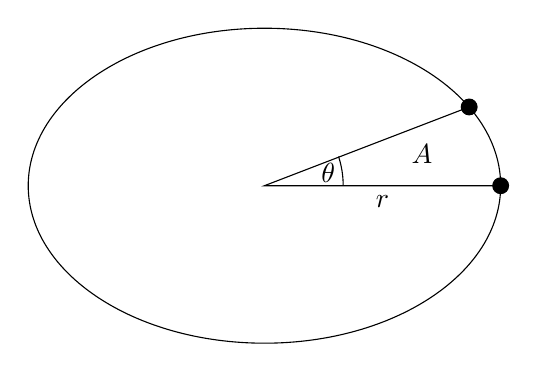
\begin{tikzpicture}[scale=2]
        \coordinate (A) at (1.5, 0);
        \coordinate (B) at (1.3, 0.5);
        \draw (0, 0) circle[x radius=1.5cm, y radius=1cm];

        \draw (A) -- (0, 0) node[pos=0.5, anchor=north] {$r$} -- (B);
        \node at (1, 0.2) {$A$};
        \node[anchor=west] at (0.3, 0.08) {$\theta$};
        \draw (0.5, 0) arc[radius=0.6cm, start angle=0, end angle=18];
        \draw[fill] (A) circle[radius=0.5mm];
        \draw[fill] (B) circle[radius=0.5mm];
    \end{tikzpicture}
    \caption{Areas swept by planetary orbit}
    \label{figOrbitAreas}
\end{figure}
The second law follows from conservation of angular momentum. In figure~\ref{figOrbitAreas}, we see that the change in area is:
\begin{equation*}
    \delta A = \frac{1}{2} r^2 \delta \theta
\end{equation*}
So the rate of change of $A$ is:
\begin{equation*}
    \dot{A} = \frac{1}{2} r^2 \dot{\theta} = \frac{1}{2}l
\end{equation*}
Which is constant since angular momentum is conserved. This also tells us that K2 is true for any central force.\par
The proof of K3 is by dimensional analysis:\par
We have $R$, the characteristic radius, and $k = GM$. Note that mass cancels. $[R] = L$, $[k] = L^3T^{-2}$. So then we have:\par
\begin{align*}
    T &\propto [R]^A [k]^B \\
    &\propto L^A L^{3B} T^{-2B}
\end{align*}
Which gives $A = \frac{3}{2}, B = -\frac{1}{2}$.\par
Therefore, we note that this only holds for central forces with potential proportional to $\frac{1}{r}$.\par
We can also fix the constant of proportionality in this equation:
\begin{align*}
    T &= \int_0^t dt = \int_0^A \frac{2}{l} dA \\
    &= \frac{2}{l} A \\
    &= \frac{2}{l} \pi a b \text{ where the semi-major and semi-minor axes are} a, b \\
    &= \frac{2\pi}{l} \frac{r_0^2}{(1-e^2)^{\frac{3}{2}}} \\
    &= \frac{2\pi}{\sqrt{k}} \frac{r_0^{\frac{3}{2}}}{(1-e^2)^{\frac{3}{2}}} \text{ since } l^2 = kr_0
\end{align*}
And if we define $R_{av} = \frac{1}{2} \left(\frac{r_0}{1+e} + \frac{r_0}{1-e}\right)$:
\begin{equation}
    T = \frac{2\pi}{\sqrt{GM}} R_{av}^{\frac{3}{2}}
    \label{eqnKepler3Improved}
\end{equation}
Thereby giving an improved version of Kepler's 3rd law.
\section{Repulsive potentials}
\begin{definition}{Scattering experiment}
    In a \underline{scattering experiment}, a particle is shot in from large $R$ at a target, and observed to fly out again at some different angle.
\end{definition}
For scattering to be possible, consider a central potential $V(r)$ which has very positive potential at small $r$, and $V(r) \to 0$ as $r \to \infty$.
\begin{definition}{Impact parameter}
    The \underline{impact parameter}, $b$, is the perpendicular distance from the target to the tangent to the initial velocity. See figure~\ref{figScatteringMotion}
\end{definition}
\begin{figure}[ht]
    \centering
    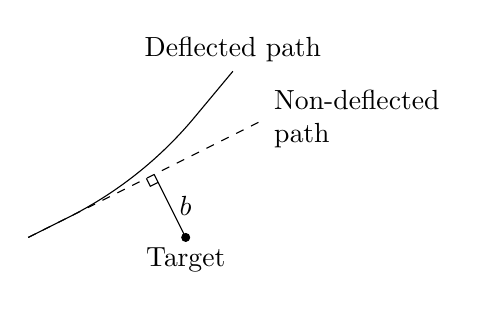
\begin{tikzpicture}
        \draw[fill] (0, 0) circle[radius=0.5mm] node[below] (T) at (0, 0) {Target};
        \coordinate (A) at (-2, 0);
        \coordinate (B) at (-1.5, 0.25);
        \coordinate (C) at (1, 1.5);
        \coordinate (D) at (-0.4, 0.8);
        \draw[dashed] (A) -- (C) node[right, align=left] {Non-deflected \\ path};
        \draw (A) -- (B) arc[radius=5cm, start angle=-63.5, end angle=-40] -- +(0.5, 0.6) node[above] {Deflected path};
        \draw (0, 0) -- (D) node[pos=0.5, anchor=west] {$b$};
        \draw (-0.5, 0.75) -- ++(0.05, -0.1) -- ++(0.1, 0.05);
    \end{tikzpicture}
    \caption{Motion of a particle in a scattering experiment}    
    \label{figScatteringMotion}
\end{figure}
The scattering parameter $b$ is related to the angular momentum $l$ by:
\begin{equation}
    l = bv
    \label{eqnScatteringAngularMomentum}
\end{equation}
We can understand this by considering a non-interacting particle, that follows the dotted trajectory in figure~\ref{figScatteringMotion}. At the point where its trajectory is a distance $b$ from the target, $l = |\vec{x} \times \dvec{x}| = b \times v$ since the vectors are orthogonal. Therefore its angular momentum at every point must be $bv$, since it is conserved.\par
Now consider an interacting particle. When the particle is infinitely far away from the target, its motion is the same as the non-interacting particle and thus its angular momentum is $bv$. This means that even when it interacts, its angular momentum is $bv$ since angular momentum is conserved.\par
We can then consider the potential around the target:
\begin{equation}
    V = \frac{K}{r} \text{ where } K = \frac{Qq}{4\pi \epsilon_0}
    \label{eqnChargePotential}
\end{equation}
Then solving the orbit equation as before:
\begin{equation}
    r = \frac{r_0}{e \cos{\theta} - 1}
    \label{eqnChargeOrbit}
\end{equation}
Now we consider the angle $\phi$ through which the particle is scattered. See figure~\ref{figScatteringAngles}.
\begin{figure}[t]
    \centering
    \begin{tikzpicture}
        \tikzset {
            patharrow/.pic={
                \draw (-0.1, 0.1) -- (0, 0) -- (0.1, 0.1);
            }
        }
        \draw[dashed] (210:3) -- (30:4);
        \draw[dashed] (150:3) -- (330:4);
        \draw[dashed] (180:2.6) -- (0:4.3);

        \draw[fill] (-1, 0) circle[radius=0.5mm];
        \draw [->] (-2, -0.3) node[anchor=north east] {Target} -- (-1.1, -0.05);

        \draw (30:5) -- (30:4) 
            arc[start angle=120, radius=2.32, end angle=240]
            pic[pos=0.3, rotate=-20] {patharrow}
            pic[pos=0.7, rotate=20] {patharrow}
            -- (330:5);

        \draw (1, 0) arc[start angle=0, end angle=30, radius=1] node[pos=0.4, anchor= east] {$\alpha$};
        \draw (1, 0) arc[start angle=0, end angle=-30, radius=1] node[pos=0.4, anchor= east] {$\alpha$};

        \draw (0.6, 0.35) arc[start angle=30, end angle=150, radius=0.7] node[pos=0.5, anchor=north] {$\phi$};

        \draw (-1, 0) -- (150:0.86) node[pos=0.7, anchor=east] {$b$};
        \draw (-1, 0) -- (210:0.86) node[pos=0.7, anchor=east] {$b$};
    \end{tikzpicture}
    \caption{Diagram of a scattering experiment with charged particles}
    \label{figScatteringAngles}
\end{figure}
Note that value of the impact parameter for the incoming and outgoing trajectories are the same due to conservation of energy and angular momentum.\par
From the diagram, $\phi = \pi - 2\alpha$. From equation~\ref{eqnChargeOrbit}, the angle $\alpha$ satisfies $\cos{\alpha} = \frac{1}{e}$. Then we can obtain $\phi$ in terms of the impact parameter and initial velocity:
\begin{align*}
    E &= \frac{1}{2}m v^2 \\
    &= \frac{k^2}{2l^2m}(e^2-1) \text{ by conservation of energy} \\
    &= \frac{k^2}{2b^2v^2m}(\tan^2{\alpha})
\end{align*}
Then substituting for $\phi$:
\begin{align*}
    \tan{\alpha} &= \tan{\left(\frac{\pi-\phi}{2}\right)} \\
    &= \frac{1}{\tan{\frac{\phi}{2}}}
\end{align*}
So then we have a formula for $\phi$:
\begin{equation}
    \phi = 2\tan^{-1} \left(\frac{k}{bmv^2}\right)
    \label{eqnScatteringAngle}
\end{equation}
Note also that for small $b$, $\phi \approx \pi$, which is the statement that the particle bounces back.
\end{document}